\chapter{Analysis}
Computational models are often too large and complex for traditional method to test, this cause developers of those models unwilling to test their models thorough. Furthermore, computational model developer are often scientist or researchers that don’t have extent knowledge in software engineering or software testing. Due to the different training receive by scientist compared to software developer, the importance of software testing is often overlooked.  \\*\\*
Causal model testing can be a powerful tool to test computational model, but causal model testing requires software testers to integrate the causal model with software model that is being tested, consider the complexity of the computational model being tested can be, it is hard to integrate the test for people who don’t have software engineering background. \\*\\*
It is possible to integrate behave and cucumber to make test computational model with causal model testing easier for people, by integrate Cucumber tester can use easy to understand language to specify the testing process and behave can read and execute these processes. By combining all these researchers who want to test their computational model can have an easy to access tool to test their software. \\*\\*
A tool with this function has already been in development for a while called Causcumber, a modify version of cucumber for testing computational model, it has the ability to use cucumber specification and behave combine with causal module testing to test computational model, but currently it still lacks an easy to use method and can only be execute in terminal with specific command. \\*\\*


\begin{center}
	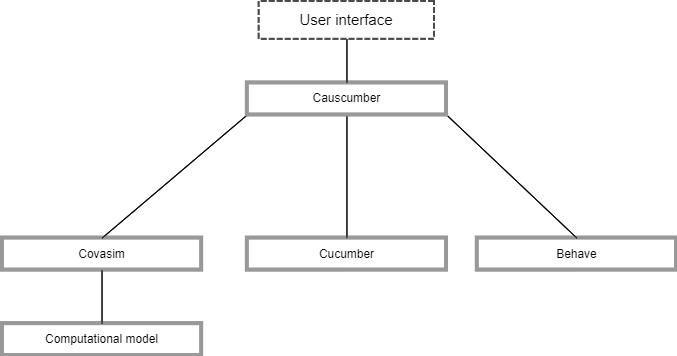
\includegraphics[width=13cm]{figures/Analysis.png}\\
	Figure 2. A diagram analysis for the system
\end{center}
\section{Project Requirements}

The main goal of this project is to develop an easy-to-use system where people can use it the execute the feature file they have written, the system will exam the feature file and go through the computational model to check if the model perform as the test specify. As a result, the system should produce a coherent result detailing the accuracy of the tested model. Thus, the systems need to accomplish the following:\\*
\\*
R1. As a user, I want this system to be easy to understand, when I use the system, I want to immediate know what I need to do to get the result I want.\\*
\\*
R2. As a user, I want the system to go through the feature file I provide and test the computational model with it.\\*
\\*
R3. As a user, I want the system to produce a result where I can know the accuracy of the computational model.\\*
\\*
Since Causcumber is already in developing for a while, what this project aims to accomplish is adding more to this tool. Currently the state of Causcumber is capable of execute some feature files that use to test a computational model named Covasim. And it is capable of returning lot of useful information, but the information still requires some organization to make the result easier to read. And currently there isn’t a way to execute the testing system without using the terminal to execute the command, so there’s a need of a user interface for people to operate the system. Last is that currently the only way to create a feature file is by hand type the files, and this might cause some error or confusion. There’s also some other requirements according to the feedback of the Causcumber team, these feedback consist of multiple function that is potent to the system and will be included during the development. Therefore, by the end of the project Causcumber should be able to accomplish the following:\\*
\\*
1.	As a user, I want the result produce by the system to be clean and easy to understand, focusing on the important part.\\*
\\*
2. As a user, I want to execute and interact with the system through a user interface.\\*
\\*
3. As a user, I want to have a more convenient way to create a feature file, to avoid any mistake during the creation of the feature file.\\*
\\*
4. As a user, I want to have the ability to toggle different types of result display for different levels of the users. \\*
\\*
5. As a user, I want to have the ability to have different input optional automatically based on different situation. \\*
\\*
6. As a user, I want to have an option to save the feature file I created. \\*
\\*

\section{Analysis}
One of the main themes for this project is ease of use, and therefore that’s what most of the requirements are focus on. For requirement R 1 – 3, the goal is to make the testing process as simple as possible, with a simplified testing process, people will be more willing to test their computational model. \\*\\*
Since integrate the causal model testing can be difficult and confusing, requirements 3, 5, 6 are focus on simplify this process, by making this part reduce to only require testers to input the parameters and their value, this should help mitigate a lot of errors. \\*\\*
Finally, this project’s main focus is on enhancing the user experience for Causcumber, this is what requirement 1, 2, 4 are for, these requirements make using Causcumber to test computational model a more convenient experience. \\*\\*

\section{Ethical, Professional and Legal Issues}

The execution of this project won’t require any real human or animal involvement, every part of this project is simulated, so there won’t be any ethical problem. All the source code used in this project are open-source and free to use, the tools used to develop the user interface are also open-source and free to use, so this mean there won’t be any legal problems either. 
